\textbf{4-1.} 面积为 $1.0\mathrm{m}^2$ 的两平行金属板，带有等量异号电荷 $\pm 30\mu \mathrm{C}$ ，其间充满了介电常量 $\varepsilon = 2.0$ 的均匀电介质。略去边缘效应，求介质内的电场强度和介质表面上的极化电荷面密度 $\sigma_{\mathrm{e}}^{\prime}$

\vfill

\textbf{4-2.} 平行板电容器(极板面积为 $S$ , 间距为 $d$ ) 中间有两层厚度各为 $d_{1}$ 和 $d_{2}(d_{1}+d_{2}=d)$ 、介电常量各为 $\varepsilon_{1}$ 和 $\varepsilon_{2}$ 的电介质层(见本题图)。试求:

(1) 电容 C;

(2) 当金属板上带电面密度为 $\pm\sigma_{e0}$ 时，两层介质的分界面上的极化电荷面密度 $\sigma_{e}^{\prime}$ ;

(3) 极板间电势差 U;

(4) 两层介质中的电位移 D.
\begin{center}
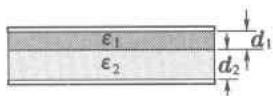
\includegraphics[width=0.3\linewidth]{figures/习题4-2.jpg}
\end{center}

\vfill
\newpage

\textbf{4-3.} 一平行板电容器两极板的面积都是 $2.0\mathrm{m}^2$ ，相距为 $5.0\mathrm{mm}$ ，两板间加上 $10000\mathrm{V}$ 电压后，取去电源，再在其间充满两层介质，一层厚 $2.0\mathrm{mm}$ 、 $\varepsilon_1 = 5.0$ ，另一层厚 $3.0\mathrm{mm}$ 、 $\varepsilon_2 = 2.0$ 。略去边缘效应，求：

(1) 各介质中的电极化强度 P;

(2) 电容器靠近电介质 2 的极板为负极板, 将它接地, 两介质接触面上的电势是多少?

\vfill

\textbf{4-4.} 平行板电容器两极板相距 $3.0\mathrm{cm}$ ，其间放有一层 $\varepsilon = 2.0$ 的电介质，位置和厚度如本题图所示。已知极板上面电荷密度为 $\sigma_{\mathrm{e0}} = 8.9\times 10^{-11}\mathrm{C / m^2}$ ，略去边缘效应，求：

(1) 极板间各处的 P、E 和 D;

(2) 极板间各处的电势(设正极板处 $U_{0}=0$ );

(3) 画 E-x、D-x、U-x 曲线；

(4) 已知极板面积为 $0.11 \, m^{2}$ ，求电容 C，并与不加电介质时的电容 $C_{0}$ 比较。
\begin{center}
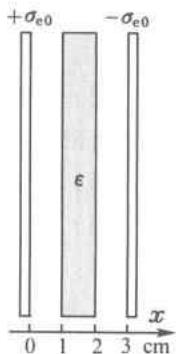
\includegraphics[width=0.15\linewidth]{figures/习题4-4.jpg}
\end{center}

\vfill
\newpage

\textbf{4-5.} 平行板电容器的极板面积为 $S$ ，间距为 $d$ ，其间充满电介质，介质的介电常量是变化的，在一极板处为 $\varepsilon_{1}$ ，在另一极板处为 $\varepsilon_{2}$ ，其它处的介电常量与到 $\varepsilon_{1}$ 处的距离呈线性关系，略去边缘效应。

(1) 求这电容器的 C;

(2) 当两极板上的电荷分别为 Q 和 -Q 时，求介质内的极化电荷体密度 $\rho_{e}^{\prime}$ 和表面上的极化电荷面密度 $\sigma_{e}^{\prime}$ .
\begin{center}
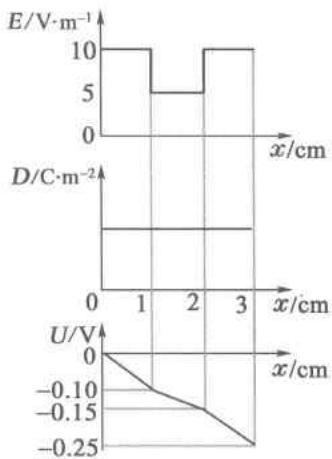
\includegraphics[width=0.3\linewidth]{figures/习题4-5.jpg}
\end{center}

\vfill

\textbf{4-6.} 一平行板电容器两极板相距为 $d$ ，其间充满了两部分介质，介电常量为 $\varepsilon_{1}$ 的介质所占的面积为 $S_{1}$ ，介电常量为 $\varepsilon_{2}$ 的介质所占的面积为 $S_{2}$ （见本题图）。略去边缘效应，求电容 $C$ .
\begin{center}
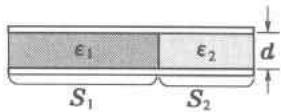
\includegraphics[width=0.3\linewidth]{figures/习题4-6.jpg}
\end{center}

\vfill
\newpage

\textbf{4-7.} 如本题图所示,一平行板电容器两极板的面积都是 S, 相距为 d, 今在其间平行地插入厚度为 t、介电常量为 $\varepsilon$ 的均匀电介质, 其面积为 S/2, 设两板分别带电荷 Q 和 -Q, 略去边缘效应, 求

(1) 两板电势差 U;

(2) 电容 C;

(3) 介质的极化电荷面密度 $\sigma_{e}^{\prime}$
\begin{center}
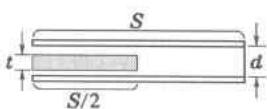
\includegraphics[width=0.3\linewidth]{figures/习题4-7.jpg}
\end{center}

\vfill

\textbf{4-8.} 同心球电容器内外半径分别为 $R_{1}$ 和 $R_{2}$ ，两球间充满介电常量为 $\varepsilon$ 的均匀电介质，内球的电荷量为 $Q$ ，求：

(1) 电容器内各处的电场强度 E 的分布和电势差 U;

(2) 介质表面的极化电荷面密度 $\sigma_{e}^{\prime}$ ;

(3) 电容 C. (它是真空时电容 $C_{0}$ 的多少倍?)

\vfill
\newpage

\textbf{4-9.} 在半径为 $R$ 的金属球之外有一层半径为 $R'$ 的均匀电介质层（见
本题图）。设电介质的介电常量为 $\varepsilon$ ，金属球带电荷量为 Q，求：

(1) 介质层内、外的场强分布；

(2) 介质层内、外的电势分布；

(3) 金属球的电势。
\begin{center}
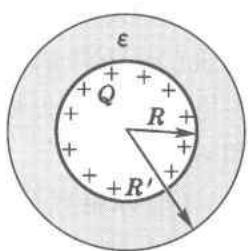
\includegraphics[width=0.25\linewidth]{figures/习题4-9.jpg}
\end{center}

\vfill

\textbf{4-10.} 一半径为 $R$ 的导体球带电荷 $Q$ , 处在介电常量为 $\varepsilon$ 的无限大均匀电介质中。求:

(1) 介质中的电场强度 E、电位移 D 和极化强度 P 的分布；

(2) 极化电荷面密度 $\sigma_{e}^{\prime}$ .

\vfill
\newpage

\textbf{4-11.} 半径为 $R$ 、介电常量为 $\varepsilon$ 的均匀介质球中心放有点电荷 $Q$ , 球外是空气。

(1) 求球内外的电场强度 E 和电势 U 的分布；

(2) 如果要使球外的电场强度为0且球内的电场强度不变，则球面上需要有面密度为多少的电荷？

\vfill

\textbf{4-12.} 球形电容器由半径为 $R_{1}$ 的导体球和与它同心的导体球壳构成，壳的内半径为 $R_{2}$ ，其间有两层均匀电介质，分界面的半径为 $r$ ，介电常量分别 $\varepsilon_{1}$ 和 $\varepsilon_{2}$ （见本题图）。

(1) 求电容 C;

(2) 当内球带电 -Q 时, 求各介质表面上极化电荷面密度 $\sigma_{e}^{\prime}$ .

\begin{center}
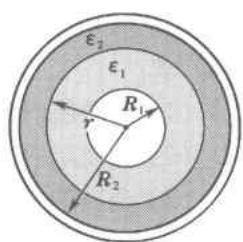
\includegraphics[width=0.3\linewidth]{figures/习题4-12.jpg}
\end{center}

\vfill
\newpage

\textbf{4-13.} 球形电容器由半径为 $R_{1}$ 的导体球和与它同心的导体球壳构成，壳的半径为 $R_{2}$ ，其间一半充满介电常量为 $\varepsilon$ 的均匀介质（见本题图）。求电容 $C$ .

\vfill

\textbf{4-14.} 圆柱形电容器是由半径为 $R_{1}$ 的导线和与它同轴的导体圆筒构成的，圆筒的内半径为 $R_{2}$ ，其间充满了介电常量为 $\varepsilon$ 的介质（见本题图）。设沿轴线单位长度上导线的电荷为 $\lambda$ ，圆筒的电荷为 $-\lambda$ ，略去边缘效应，求：

(1) 两极的电势差 U;

(2) 介质中的电场强度 E、电位移 D、极化强度 P;

(3) 介质表面的极化电荷面密度 $\sigma_{e}^{\prime}$ ;

(4) 电容 C. (它是真空时电容 $C_{0}$ 的多少倍?)
\begin{center}
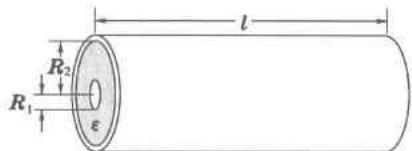
\includegraphics[width=0.3\linewidth]{figures/习题4-14.jpg}
\end{center}


\vfill
\newpage

\textbf{4-15.} 圆柱形电容器是由半径为 $a$ 的导线和与它同轴的导电圆筒构成，圆筒内半径为 $b$ ，长为 $l$ ，其间充满了两层同轴圆筒形的均匀电介质，分界面的半径为 $r$ ，介电常量分别为 $\varepsilon_{1}$ 和 $\varepsilon_{2}$ （见本题图），略去边缘效应，求电容 $C$ .
\begin{center}
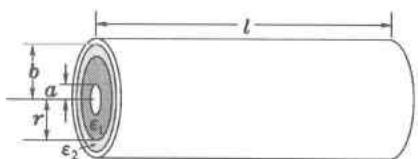
\includegraphics[width=0.3\linewidth]{figures/习题4-15.jpg}
\end{center}

\vfill

\textbf{4-16.} 一长直导线半径为 $1.5\mathrm{cm}$ , 外面套有内半径为 $3.0\mathrm{cm}$ 的导体圆筒, 两者共轴。当两者电势差为 $5000\mathrm{V}$ 时, 何处电场强度最大? 其值是多少?与其间介质有无关系？

\vfill
\newpage

\textbf{4-17.} 求垂直轴线均匀极化的无限长圆柱形电介质轴线上的退极化场，已知极化强度为 $P$

\vfill

\textbf{4-18.} 在介电常量为 $\varepsilon$ 的无限大均匀电介质中存在均匀电场 $E_0$ . 今设想以其中某点 $O$ 为中心作一球面, 把介质分为内、外两部分。求球面外全部电荷在 $O$ 点产生的场强 $E$ . (E 比 $E_0$ 大还是小?)

\vfill
\newpage

\textbf{4-19.} 在介电常量为 $\varepsilon$ 的无限大均匀电介质中存在均匀电场 $E_0$ . 今设想在其中作一轴线与 $E_0$ 垂直的无限长圆柱面, 把介质分为内、外两部分。求柱面外全部电荷在柱轴上产生的场强 $E$ . (如果真把圆柱面内部的介质挖去, 本题的结论还适用吗?)

\vfill

\textbf{4-20.} 空气的介电强度为 $3.0 \times 10^{6} \mathrm{~V} / \mathrm{m}$ , 铜的密度为 $8.9 \mathrm{~g} / \mathrm{cm}^{3}$ , 铜的原子量为 $63.75 \mathrm{~g} / \mathrm{mol}$ , 阿伏伽德罗常量 $N_{\mathrm{A}} = 6.022 \times 10^{23} \mathrm{~mol}^{-1}$ , 金属铜里每个铜原子有一个自由电子, 每个电子的电荷量为 $1.60 \times 10^{-19} \mathrm{C}$ .

(1) 问半径为 $1.0 \, cm$ 的铜球在空气中最多能带多少电荷量？

(2) 这铜球所带电荷量达到最多时，求它所缺少或多出的电子数与自由电子总数之比；

(3) 因导体带电时电荷都在外表面上，当铜球所带电压达到最多时，求它所缺少或多出的电子数与表面一层铜原子所具有的自由电子数之比。

【提示:可认为表面层的厚度为 $n^{-1/3}$ ，n 为原子数密度。】


\vfill
\newpage

\textbf{4-22.} 一圆柱形电容器,由直径为 $5.0 \mathrm{~cm}$ 的直圆筒和与它共轴的直导线构成,导线的直径为 $5.0 \mathrm{~mm}$ ,筒与导线间是空气,已知空气的击穿场强为 $30000 \mathrm{~V} / \mathrm{cm}$ ,问这电容器能耐多高的电压?

\vfill

\textbf{4-23.} 两共轴的导体圆筒，内筒外半径为 $R_{1}$ ，外筒内半径为 $R_{2}$ ( $R_{2} < 2R_{1}$ )，其间有两层均匀介质，分界面的半径为 $r$ ，内层介电常量为 $\varepsilon_{1}$ ，外层介电常量为 $\varepsilon_{2} = \varepsilon_{1}/2$ ，两介质的介电强度都是 $E_{\max}$ .

(1) 当电压升高时, 哪层介质先击穿?

(2) 证明: 两筒最大的电势差为
$$
U _ {\max} = \frac {E _ {\max} r}{2} \ln \frac {R _ {2} ^ {2}}{r R _ {1}}.
$$

\vfill
\newpage

\textbf{4-24.} 设一同轴电缆里面导体的半径是 $R_{1}$ ，外面的半径是 $R_{3}$ ，两导体间充满了两层均匀电介质，它们的分界面的半径是 $R_{2}$ ，设内外两层电介质的介电常量分别为 $\varepsilon_{1}$ 和 $\varepsilon_{2}$ （横截面见本题图），它们的介电强度分别为 $E_{1}$ 和 $E_{2}$ ，证明：当两极（即两导体）间的电压逐渐升高时，在$\varepsilon_ {1} E _ {1} R _ {1} > \varepsilon_ {2} E _ {2} R _ {2}$
的条件下,首先被击穿的是外层电介质。

\begin{center}
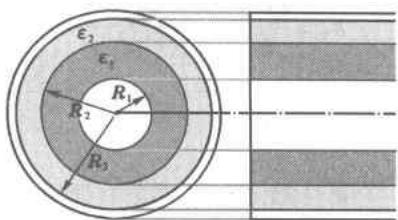
\includegraphics[width=0.3\linewidth]{figures/习题4-24.jpg}
\end{center}

\vfill

\textbf{4-25.} 一均匀磁化的磁棒，直径为 $25\mathrm{mm}$ ，长为 $75\mathrm{mm}$ ，磁矩为 $12000\mathrm{A} \cdot \mathrm{m}^2$ ，求棒侧表面上的面磁化电流密度。

\vfill
\newpage

\textbf{4-26.} 一均匀磁化磁棒,体积为 $0.01\mathrm{m}^3$ ,磁矩为 $500\mathrm{A}\cdot \mathrm{m}^2$ ，棒内的磁感应强度 $B = 5.0\mathrm{Gs}$

(1) 求磁场强度为多少 Oe;

(2) 按照磁荷观点, 磁棒端面上磁荷密度和磁极化强度为多少?

\vfill

\textbf{4-27.} 一长螺线管长为 $l$ ，由表面绝缘的导线密绕而成，共绕有 $N$ 匝，导线中通有电流 $I$ . 一同样长的铁磁棒，横截面也和上述螺线管相同，棒是均匀磁化的，磁化强度为 $M$ ，且 $M = NI / l$ . 在同一坐标纸上分别以该螺线管和铁磁棒的轴线为横坐标 $x$ ，以它们轴线上的 $B, \mu_0 M$ 和 $\mu_0 H$ 为纵坐标，画出包括螺线管和铁磁棒在内两倍长度区间的 $B - x, \mu_0 M - x$ 和 $\mu_0 H - x$ 曲线。

\vfill
\newpage

\textbf{4-28.} 一圆柱形永磁铁, 直径 $10 \mathrm{~mm}$ , 长 $100 \mathrm{~mm}$ , 均匀磁化后磁极化强度 $J = 1.20 \mathrm{~Wb} / \mathrm{m}^{2}$ , 求:

(1) 它两端的磁荷密度；

(2) 它的磁矩；

(3) 其中心的磁场强度 H 和磁感应强度 B. 此外, H 和 B 的方向关系若何?

\vfill

\textbf{4-29.} (1) 一圆磁片半径为 $R$ ，厚为 $l$ ，片的两面均匀分布着磁荷，面密度分别为 $\sigma_{\mathrm{m}}$ 和 $-\sigma_{\mathrm{m}}$ （见本题图）。求轴线上离圆心为 $x$ 处的磁场强度 $H$

(2) 此磁片的磁偶极矩 $p_{m}$ 和磁矩 m 为多少?

(3) 试证明，当 $l \ll R$ （磁片很薄）时，磁片外轴线上的磁场分布与一个磁矩和半径相同的电流环所产生的磁场一样。
\begin{center}
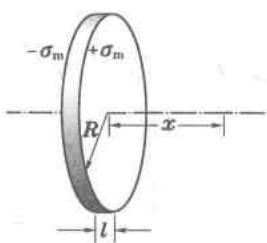
\includegraphics[width=0.3\linewidth]{figures/习题4-29.jpg}
\end{center}

\vfill
\newpage

\textbf{4-30.} 地磁场可以近似地看作是位于地心的一个磁偶极子产生的，在地磁纬度 $45^{\circ}$ 处，地磁的水平分量平均为0.23Oe，地球的平均半径为6370km，求上述磁偶极子的磁矩。

\vfill

\textbf{4-31.} 地磁场可以近似地看做是位于地心的一个磁偶极子产生的。证明：磁倾角（地磁场的方向与当地水平面之间的夹角） $i$ 与地磁纬度 $\varphi$ 的关系为（见本题图）$\tan i = 2 \tan \varphi .$
\begin{center}
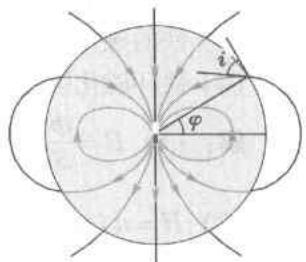
\includegraphics[width=0.3\linewidth]{figures/习题4-31.jpg}
\end{center}

\vfill
\newpage

\textbf{4-32.} 根据测量得出,地球的磁矩为 $8.4 \times 10^{22} \mathrm{~A} \cdot \mathrm{m}^{2}$ .
(1) 如果在地磁赤道上套一个铜环，在铜环中通以电流 I，使它的磁矩等于地球的磁矩，求 I 的值（已知地球半径为 6370 km）；

(2) 如果这电流的磁矩正好与地磁矩的方向相反，这样能不能抵消地球表面的磁场？


\vfill

\textbf{4-33.} 一环形铁芯横截面的直径为 $4.0\mathrm{mm}$ , 环的平均半径 $R = 15\mathrm{mm}$ , 环上密绕着200匝线圈（见本题图）, 当线圈导线通有 $25\mathrm{mA}$ 的电流时, 铁芯的磁导率 $\mu = 300$ , 求通过铁芯横截面的磁通量 $\Phi$ .

\vfill
\newpage

\textbf{4-34.} 一铁环中心线的周长为 $30\mathrm{cm}$ ，横截面积为 $1.0\mathrm{cm}^2$ ，在环上紧密地绕有300匝表面绝缘的导线，当导线中通有电流 $32\mathrm{mA}$ 时，通过环的横截面的磁通量为 $2.0\times 10^{-6}\mathrm{Wb}$ ，求：

(1) 铁环内部磁感应强度的大小 B;

(2) 铁环内部磁场强度的大小 H;

(3) 铁的磁化率 $\chi_{m}$ 和磁导率 $\mu$ ;

(4) 铁环磁化强度的大小 M.

\vfill

\textbf{4-35.} 一无穷长圆柱形直导线外包一层磁导率为 $\mu$ 的圆筒形磁介质，导线半径为 $R_{1}$ ，磁介质的外半径为 $R_{2}$ （见本题图），导线内有电流 $I$ 通过。

(1) 求介质内、外的磁场强度和磁感应强度的分布，并画 H-r 和 B-r 曲线；

(2) 介质内、外表面的磁化面电流密度 $i'$ ;

(3) 从磁荷观点来看, 磁介质表面有无磁荷?
\begin{center}
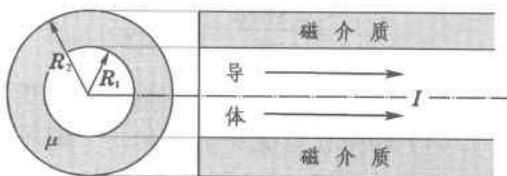
\includegraphics[width=0.4\linewidth]{figures/习题4-35.jpg}
\end{center}
\vfill
\newpage

\textbf{4-36.} 本题图是某种铁磁材料的起始磁化曲线，试根据这曲线求出最大磁导率 $\mu_{\text{最大}}$ ，并绘制相应的 $\mu - H$ 曲线。

\begin{center}
    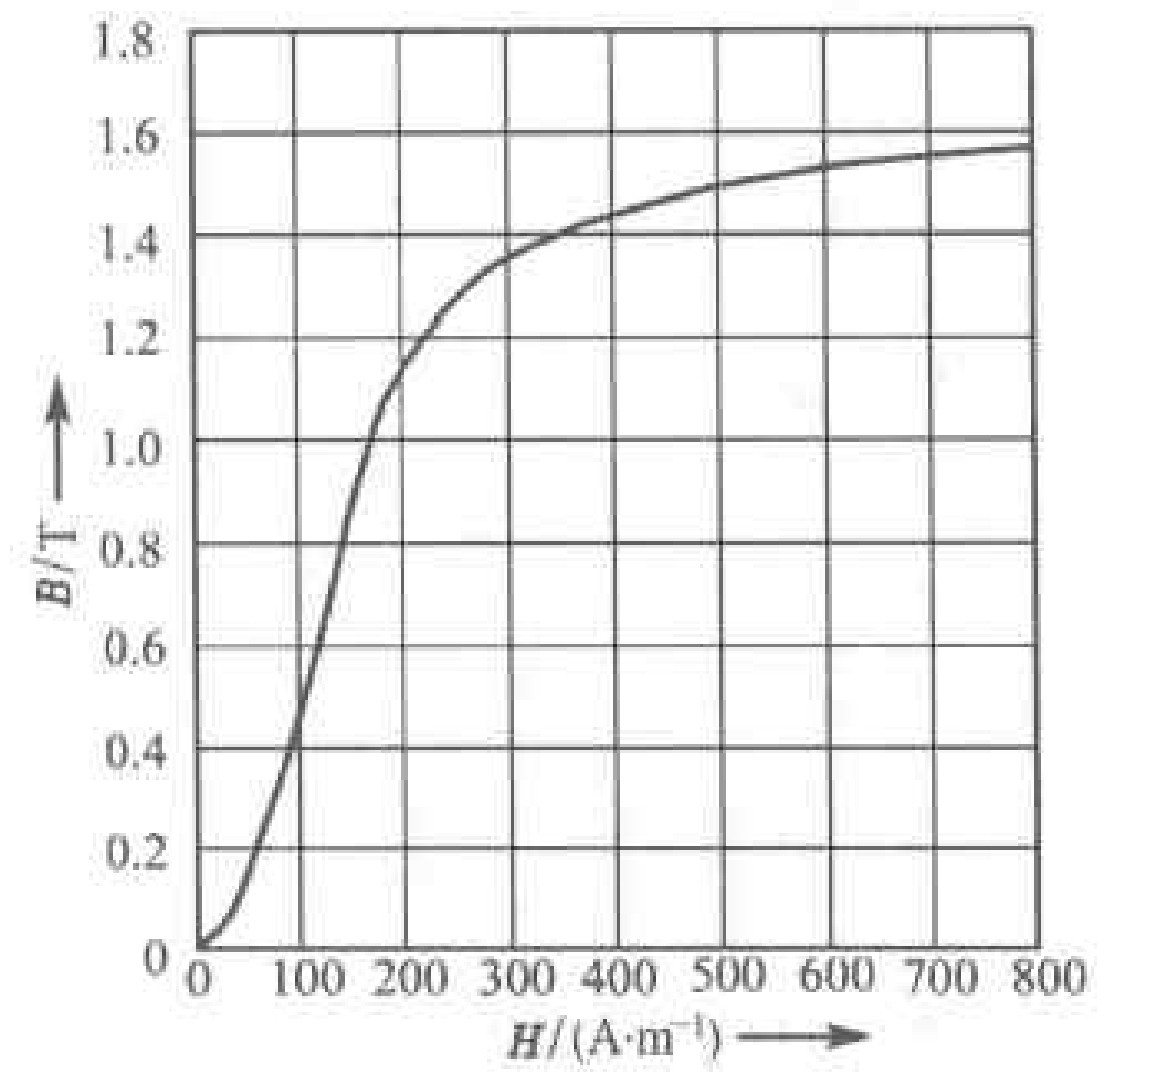
\includegraphics[width = 0.3\linewidth]{figures/习题4-36.jpg}
\end{center}

\vfill

\textbf{4-37.} 下表中列出某种磁性材料的 $H$ 和 $B$ 的实验数据，
\begin{center}
    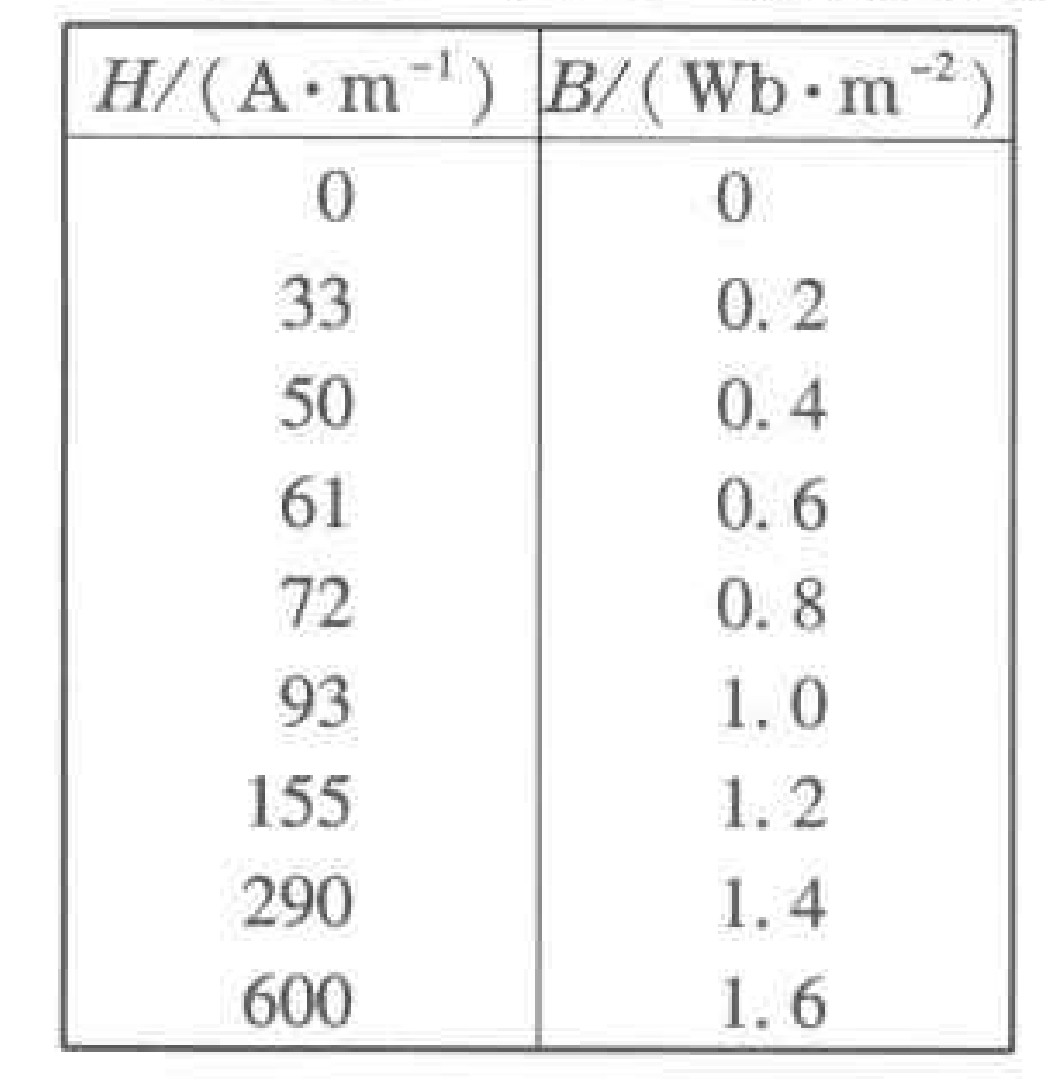
\includegraphics[width = 0.3\linewidth]{figures/习题4-37.jpg}
\end{center}
(1) 画出此材料的起始磁化曲线；

(2) 求表中所列各点处材料的磁导率 $\mu$ ;

\vfill
\newpage

\textbf{4-38.} 中心线周长为 $20\mathrm{cm}$ 、截面积为 $4\mathrm{cm}^2$ 的闭合环形磁芯，其材料的磁化曲线如本题图所示。

(1) 若需要在该磁芯中产生磁感强度为0.1、0.6、1.2、 $1.8\ Wb/m^{2}$ 的磁场时, 绕组的A·匝数NI要多大?

(2) 若绕组的匝数 N=1000，上述各种情况下通过绕组的电流 I 应多大？

(3) 若固定绕组中的电流, 使它恒为 I=0.1A, 绕组的匝数各为多少?

(4) 求上述各工作状态下材料的磁导率 $\mu$ .
\begin{center}
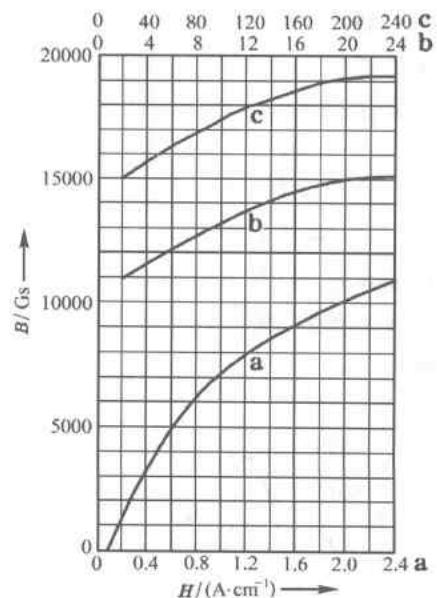
\includegraphics[width=0.3\linewidth]{figures/习题4-38.jpg}
\end{center}


\vfill

\textbf{4-39.} 矩磁材料具有矩形磁滞回线（见本题图a），反向场一超过矫顽力，磁化方向就立即反转。矩磁材料的用途是制作电子计算机中存储元件的环形磁芯。图b所示为一种这样的磁芯，其外直径为 $0.8\mathrm{mm}$ ，内直径为 $0.5\mathrm{mm}$ ，高为 $0.3\mathrm{mm}$ ，这类磁芯由矩磁铁氧体材料制成。若磁芯原来已被磁化,其方向如图所示。现需使磁芯中自内到外的磁化方向全部翻转,导线中脉冲电流 i 的峰值至少需多大?设磁芯矩磁材料的矫顽力 $H_{C}=2Oe$ .
\begin{center}
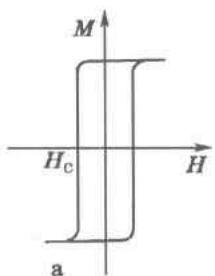
\includegraphics[width=0.2\linewidth]{figures/习题4-39.jpg}
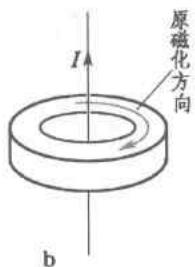
\includegraphics[width=0.2\linewidth]{figures/习题4-39b.jpg}
\end{center}

\vfill
\newpage

\textbf{4-40.} 在空气 $(\mu = 1)$ 和软铁 $(\mu = 7000)$ 的交界面上，软铁内的磁感强度 $B$ 与交界面法线的夹角为 $85^{\circ}$ ，求空气中磁感强度与交界面法线的夹角。

\vfill

\textbf{4-41.} 一铁芯螺绕环由表面绝缘的导线在铁环上密绕而成，环的中心线长 $500\mathrm{mm}$ ，横截面积为 $1000\mathrm{mm}^2$ 。现在要在环内产生 $B = 1.0\mathrm{T}$ 的磁感应强度，由铁的 $B - H$ 曲线得这时铁的 $\mu = 796$ ，求所需的A·匝数NI。如果铁环上有一个 2.0 mm 宽的空气间隙, 所需的 A·匝数 NI 又为多少?

\vfill
\newpage

\textbf{4-42.} 一铁环中心线的半径 $R = 200\mathrm{mm}$ ，横截面积为 $150\mathrm{mm}^2$ ，在它上面绕有表面绝缘的导线 $N$ 匝，导线中通有电流 $I$ ，环上有一个 $1.0\mathrm{mm}$ 宽的空气隙。现在要在空气隙内产生 $B = 0.50\mathrm{T}$ 的磁感应强度，由铁的 $B - H$ 曲线得这时铁的 $\mu = 250$ ，求所需的A·匝数 $NI$ 。


\vfill

\textbf{4-43.} 一铁环中心线的直径 $D = 40\mathrm{cm}$ ，环上均匀地绕有一层表面绝缘的导线，导线中通有一定电流。若在这环上锯一个宽为 $1.0\mathrm{mm}$ 的空气隙，则通过环的横截面的磁通量为 $3.0\times 10^{-4}\mathrm{Wb}$ ；若空气隙的宽度为 $2.0\mathrm{mm}$ ，则通过环的横截面的磁通量为 $2.5\times 10^{-4}\mathrm{Wb}$ ，忽略漏磁不计，求这铁环的磁导率。


\vfill
\newpage

\textbf{4-44.} 一铁环中心线的半径 $R = 20\mathrm{cm}$ ，横截面是边长为 $4.0\mathrm{cm}$ 的正方形。环上绕有500匝表面绝缘的导线。导线中载有电流1.0A，这时铁的磁导率 $\mu = 400$

(1) 求通过环的横截面的磁通量；

(2) 如果在这环上锯开一个宽为1.0mm的空气隙，求这时通过环的横截面的磁通量的减少。

\vfill

\textbf{4-45.} 一个利用空气间隙获得强磁场的电磁铁如本题图所示，铁芯中心线的长度 $l_{1} = 500\mathrm{mm}$ ，空气隙长度 $l_{2} = 20\mathrm{mm}$ ，铁芯是磁导率 $\mu = 5000$ 的硅钢。要在空气隙中得到 $B = 3000$ Gs 的磁场，求绕在铁芯上的线圈的 A·匝数 $NI$ .
\begin{center}
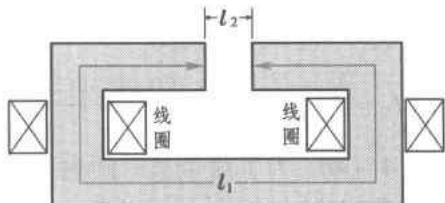
\includegraphics[width=0.3\linewidth]{figures/习题4-45.jpg}
\end{center}

\vfill
\newpage

\textbf{4-46.} 某电钟里有一铁芯线圈，已知铁芯磁路长 $14.4\mathrm{cm}$ ，空气隙宽 $2.0\mathrm{mm}$ ，铁芯横截面积为 $0.60\mathrm{cm}^2$ ，钦芯的磁导率 $\mu = 1600$ 。现在要使通过空气隙的磁通量为 $4.8\times 10^{-6}\mathrm{Wb}$ ，求线圈电流的A·匝数NI。若线圈两端电压为 $220\mathrm{V}$ ，线圈消耗的功率为 $2.0\mathrm{W}$ ，求线圈的匝数N。


\vfill

\textbf{4-47.} 本题图是某日光灯所用镇流器铁芯尺寸（单位为 $\mathrm{mm}$ ），材料的磁化曲线见习题4-41附图。在铁芯上共绕 $N = 1280$ 匝线圈，现要求线圈中通过电流 $I = 0.41\mathrm{A}$ 时铁芯中的磁通量 $\Phi = 5.8\times 10^{-4}\mathrm{Wb}$ ，

(1) 求此时气隙中的磁感应强度和磁场强度；

(2) 求铁芯中的磁感应强度 B 和磁场强度 H;

(3) 应留多大的气隙才能满足上述要求?
\begin{center}
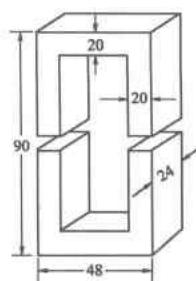
\includegraphics[width=0.2\linewidth]{figures/习题4-47.jpg}
\end{center}

\vfill
\newpage

\textbf{4-48.} 为了测量某一硬磁材料的磁棒的磁滞回线,需要测量其中磁场强度 $H$ 的变化。为此将磁棒夹在电磁铁的两极之间,用平均直径为 $D$ 的半圆形有机玻璃为芯做一磁势计,放在硬磁棒侧面上(见本题图)。

(1) 磁势计测得的磁势降落与磁棒内的磁场强度 H 有什么关系?

(2) 先增加电磁铁绕组中的电流 I 使硬磁棒的磁化达到饱和, 然后将励磁电流突然切断, 由冲击电流计测得迁移的电量 $q = 25 \mu C$ , 已知半圆磁势计的平均直径 D = 1.6 cm, 横截面积 $S = 0.16 cm^{2}$ , 磁势计线圈共有 3725 匝, 电路的总电阻 $R = 4100 \Omega$ , 求硬磁棒中的磁场强度 H 的改变量。(切断励磁电流后, 硬磁棒内的磁场强度是否为 0? 为什么?)
\begin{center}
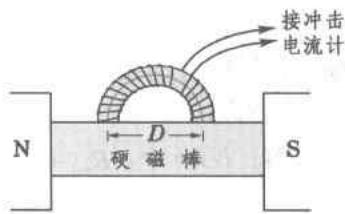
\includegraphics[width=0.3\linewidth]{figures/习题4-48.jpg}
\end{center}

\vfill

\textbf{4-49.} 电视显像管的磁偏转线圈套在管颈上，在管颈中间产生一个均匀磁场。磁偏转线圈的结构如本题图a所示，用磁性材料做一个空心磁环，把线缠绕在上面， $A、A'$ 处绕得较稀， $B、B'$ 处绕得较密，而且 $ABA'$ 与 $AB'A'$ 两半边绕
\begin{center}
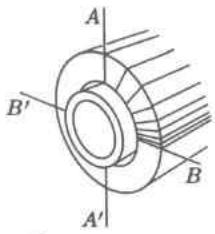
\includegraphics[width=0.2\linewidth]{figures/习题4-49.jpg}
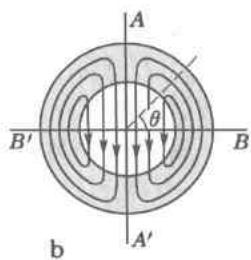
\includegraphics[width=0.2\linewidth]{figures/习题4-49b.jpg}
\end{center}
的方向相反(图 a 中只画了一个象限内的绕组)。于是磁感应线就会形成如图 b 的均匀分布。设磁芯的磁导率很大，从而其中磁阻可以忽略。试证明，为了在管颈中得到均匀磁场，磁环单位长度上线圈的匝数应服从下列规律：
$$
n (\theta) \propto \cos \theta .
$$
其中 $\theta$ 是从 B 点算起的方位角。

\vfill\newpage

\textbf{4-50.} (1) 证明电磁铁吸引衔铁的起重力 $F$ （见本题图）为 $F = \frac{SB^2}{2\mu_0}$
式中 S 为两磁极与衔铁相接触的总面积，B 为电磁铁内的磁感应强度（设磁铁内的 $H \ll M$ ）。

(2) 起重力与磁极、衔铁间的距离 x 有无关系?
【提示:先假设衔铁与磁极之间有长度为 x 的小气隙，则磁极和衔铁的表面带有正、负号相反的磁荷，起重力，即它们之间的吸引力为$F = \frac {1}{2} S \sigma_ {\mathrm{m}} H,$式中H为气隙中的磁场强度。(为什么有因子1/2?) 进一步用磁铁内部的B将 $\sigma_{m}$ 、H表示出来,即可得到上述公式。令 $x\rightarrow0$ ,可以计算衔铁与磁极直接接触时的相互作用力,即最大的起重力。
\begin{center}
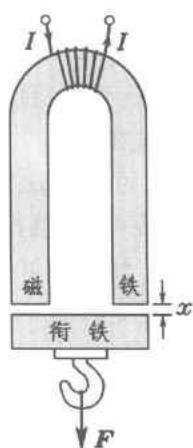
\includegraphics[width=0.13\linewidth]{figures/习题4-50.jpg}
\end{center}


\vfill
\textbf{4-51.} 在上题中已知电磁铁的每个磁极的面积都是 $1.5 \times 10^{-2} \mathrm{~m}^2$ 。在磁极与衔铁间夹有薄铜片，以免铁与铁直接接触。设这时的磁通量为 $1.5 \times 10^{-2} \mathrm{~Wb}$ ，求这电磁铁的起重力。

\vfill\newpage

\textbf{4-52.} (1)一起重用的马蹄形电磁铁形状如本题图所示，两极的横截面都是边长为 $a$ 的正方形，磁铁的磁导率 $\mu = 200$ ，上面绕有 $N = 200$ 匝线圈，电流 $I = 2.0\mathrm{A}$ ，已知 $R = a = x = 5.0\mathrm{cm}, l = d = 10\mathrm{cm}$ 衔铁与磁极直接接触。求这电磁铁的起重力（包括衔铁在内）。

(2) 若磁铁与衔铁间垫有厚 1.0 mm 的铜片, 当负重(包括衔铁自重)20 kg 时, 需要多大电流?
\begin{center}
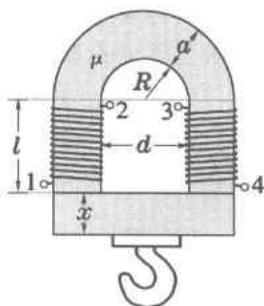
\includegraphics[width=0.3\linewidth]{figures/习题4-52.jpg}
\end{center}
\vfill


\textbf{4-53.} (1) 在上题中两绕组串联和并联时，1、2、3、4各接头该如何连接？

(2) 若两绕组完全相同, 在同样电压的条件下, 哪种连接方法使电磁铁的起重力较大? 大几倍?

(3) 在同样电流的条件下比较, 结论如何?

(4) 在同样功率的条件下比较, 结论如何?

\vfill\newpage

\textbf{4-54.} 一磁铁棒长 $5.0\mathrm{cm}$ , 横截面积为 $1.0\mathrm{cm}^2$ , 设棒内所有铁原子的磁矩都沿棒长方向整齐排列, 每个铁原子的磁矩为 $1.8 \times 10^{-23}\mathrm{A} \cdot \mathrm{m}^2$ .

(1) 求这磁铁棒的磁矩 m 和磁偶极矩 $p_{m}$ ;

(2) 当这磁铁棒在 $B = 1.5\mathrm{Gs}$ 的外磁场中并与之垂直时， $\pmb{B}$ 使它转动的力矩有多大？

\vfill


\textbf{4-55.} 一磁针的磁矩为 $20\mathrm{A}\cdot \mathrm{m}^2$ ，处在 $B = 5.0\times 10^{-2}\mathrm{Gs}$ 的均匀外磁场中。求 $B$ 作用在这磁针上的力矩的最大值。

\vfill\newpage

\textbf{4-56.} 一小磁针的磁矩为 $m$ ，处在磁场强度为 $\pmb{H}$ 的均匀外磁场中，这磁针可以绕它的中心转动，转动惯量为 $J$ . 它在平衡位置附近作小振动时，求振动的周期和频率。

\vfill


\textbf{4-57.} 两磁偶极排列在同一条直线上，它们的磁偶极矩分别为 $p_{\mathrm{m1}}$ 和 $p_{\mathrm{m2}}$ ，中心的距离为 $r$ ，它们各自的长度都比 $r$ 小很多。

(1) 证明：它们之间相互作用力是大小 $F = \dfrac{3p_{\mathrm{m1}}p_{\mathrm{m2}}}{2\pi\mu_0r^4}$

(2) 在什么情况下它们互相吸引? 在什么情况下互相排斥?

\vfill\newpage

\textbf{4-58.} 一抗磁质小球的质量为 $0.10\mathrm{g}$ ，密度 $\rho = 9.8\mathrm{g/cm^3}$ ，磁化率 $\chi_{\mathrm{m}} = -1.82\times 10^{-4}$ ，放在一个半径 $R = 10\mathrm{cm}$ 的圆线圈的轴线上距圆心 $l = 10\mathrm{cm}$ 处（见本题图），线圈中载有电流 $I = 1.0\mathrm{mA}$ 。求电流作用在这抗磁质小球上的力的大小和方向。
\begin{center}
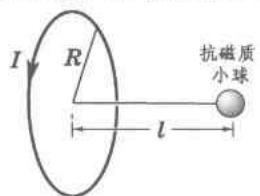
\includegraphics[width=0.3\linewidth]{figures/习题4-58.jpg}
\end{center}

\vfill


\textbf{4-59.} 一平行板电容器极板面积为 $S$ ，间距为 $d$ ，电荷为 $\pm Q$ . 将一块厚度为 $d$ 、介电常量为 $\varepsilon$ 的均匀电介质板插入极板间空隙。计算：

(1) 静电能的改变；

(2) 电场力对介质板作的功。

\vfill\newpage

\textbf{4-60.} 一平行板电容器极板面积为 $S$ ，间距为 $d$ ，接在电源上以维持其电压为 $U$ 。将一块厚度为 $d$ 、介电常量为 $\varepsilon$ 的均匀电介质板插入极板间空隙。计算：

(1) 静电能的改变；

(2) 电源所作的功；

(3) 电场对介质板作的功。

\vfill


\textbf{4-61.} 一平行板电容器极板是边长为 $a$ 的正方形，间距为 $d$ ，电荷 $\pm Q$ 把一块厚度为 $d$ 、介电常量为 $\varepsilon$ 的电介质板插入一半，它受力多少？什么方向？

\vfill\newpage

\textbf{4-62.} 两个相同的平行板电容器, 它们的极板都是圆形的, 半径 $10 \mathrm{~cm}$ , 极板间隔 $1.0 \mathrm{~mm}$ . 两电容器中一个两板间是空气, 另一个两板间是 $\varepsilon = 26$ 的酒精。把这两个电容器并联后充电到 $120 \mathrm{~V}$ , 求它们所蓄的总电能; 再断开电源, 把它们带异号电荷的两极分别联在一起, 求这时两者所蓄的总电能。少的能量哪里去了?

\vfill


\textbf{4-63.} 球形电容器的内外半径分别为 $R_{1}$ 和 $R_{2}$ , 电势差为 $U$ .

(1) 求电容器所储的静电能；

(2) 求电场的能量; 比较两个结果。

\vfill\newpage

\textbf{4-64.} 半径为 $a$ 的导体圆柱外面套有一半径为 $b$ 的同轴导体圆筒，长度都是 $l$ ，其间充满介电常量为 $\varepsilon$ 的均匀介质。圆柱带电为 $Q$ ，圆筒带电为 $-Q$ ，略去边缘效应。

(1) 整个介质内的电场总能量 $W_{e}$ 是多少?

(2) 证明： $W_{e}=\frac{1}{2}\frac{Q^{2}}{C}$ ，式中 C 是圆柱和圆筒间的电容。

\vfill


\textbf{4-65.} 圆柱电容器由一长直导线和套在它外面的共轴导体圆筒构成。设导线的半径为 $a$ ，圆筒的内半径为 $b$ 。证明：这电容器所储藏的能量有一半是在半径 $r = \sqrt{ab}$ 的圆柱体内。

\vfill\newpage

\textbf{4-66.} 目前在实验室里产生 $E = 10^{5} \mathrm{~V} / \mathrm{m}$ 的电场和 $B = 10^{4} \mathrm{Gs}$ 的磁场是不难做到的。今在边长为 $10 \mathrm{~cm}$ 的立方体空间里产生上述两种均匀场，问所需的能量各为多少？


\vfill


\textbf{4-67.} 利用高磁导率的铁磁体，在实验室产生 $B = 5000\mathrm{Gs}$ 的磁场并不困难。

(1) 求这磁场的能量密度 $w_{m}$ ;

(2) 要想产生能量密度等于这个值的电场，问电场强度 E 的值应为多少？这在实验中容易做到吗？

\vfill\newpage

\textbf{4-68.} 一同轴线由很长的直导线和套在它外面的同轴圆筒构成，导线的半径为 $a$ ，圆筒的内半径为 $b$ ，外半径为 $c$ ，电流 $I$ 沿圆筒流去，沿导线流回；在它们的横截面上电流都是均匀分布的。

(1) 求下列四处每米长度内所储磁能 $W_{m}$ 的表达式：导线内，导线和圆筒之间，圆筒内，圆筒外；

(2) 当 $a=1.0\ mm,\ b=4.0\ mm,\ c=5.0\ mm,\ I=10A$ 时，每米长度的同轴线中储存磁能多少？

\vfill


\textbf{4-69.} 试验算一下，用7.2节所述两种平均磁链法计算例题18的结果，都与磁能法一致。

\vfill
\newpage